\documentclass[20pt]{beamer}
\usepackage[]{bookmark}
\usepackage[utf8]{inputenc}
\usepackage{amsmath}
\usepackage{amsfonts}
\usepackage{amssymb}
\usepackage{tikz}
\usepackage{xcolor}
\usepackage[dutch]{babel}
\usepackage{sansmathaccent}
\usepackage{graphicx}

\usepackage[style=authoryear,backend=biber]{biblatex}

\addbibresource{bibliography2.bib} 
\pdfmapfile{+sansmathaccent.map}

\title{RMC voor lineaire ODEs}
\author{Isidoor Pinillo Esquivel }
\usetheme{Madrid}
\date{}

\begin{document}

% 1 min
\begin{frame}
    \titlepage
\end{frame}
% 2 min
\begin{frame}
    \frametitle{Grid-Free Monte Carlo}
    \cite{sawhney_grid-free_2022}
    \begin{figure}[h!]
        \centering
        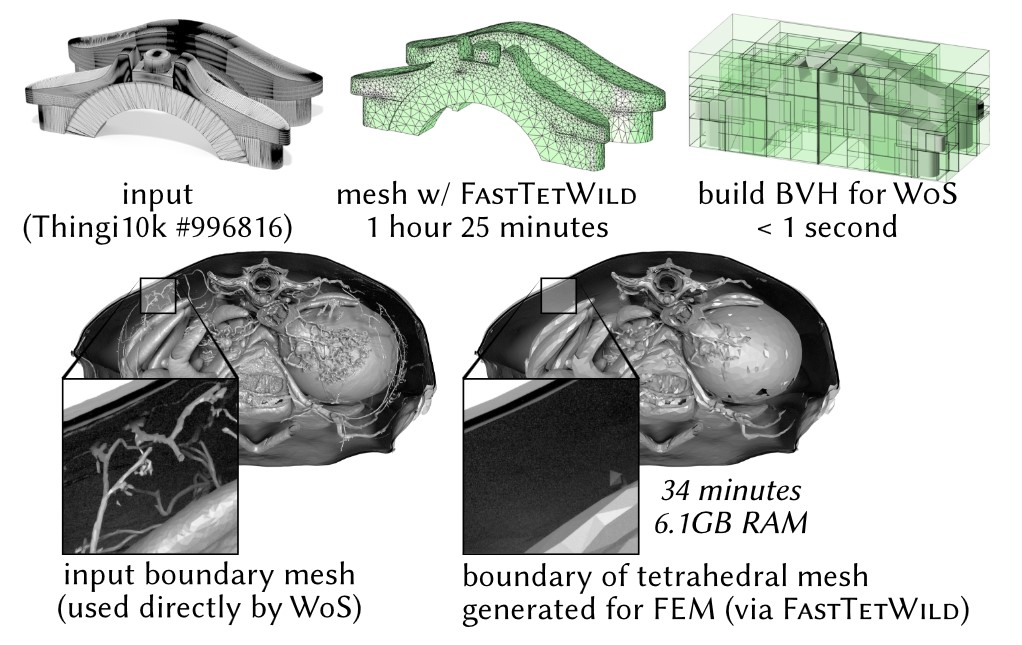
\includegraphics[width=0.8\textwidth]{imgs/Grid_free_comparison.jpg}
        \label{fig:grid_free_comparison}
    \end{figure}
\end{frame}

% 2 min
\begin{frame}
    \frametitle{Monte Carlo}
    \vspace{-1cm}
    \begin{align}
        \int_{0}^{1} f(x) dx & = E[f(U)]                                   \\
                             & \approx \frac{1}{n} \sum_{j=1}^{n} f(U_{j})
    \end{align}
    \begin{center}
        met $U_{j} \sim \text{Uniform}(0,1)$
    \end{center}
\end{frame}

\begin{frame}
    \frametitle{Waarom Monte Carlo?}
    \begin{itemize}
        \item eenvoudig
        \item paralleliseerbaar
        \item dimensie onafhankelijke convergentie
        \item complexe geometrie
        \item enkel simulaties beschikbaar
    \end{itemize}
\end{frame}

\begin{frame}
    \frametitle{Waarom ODEs?}
    \begin{itemize}
        \item grid-free + tijdafhankelijkheid
        \item ODEs simpeler als PDEs
    \end{itemize}
\end{frame}

\begin{frame}
    \frametitle{Stochastic Gradient Descent}
    \vspace*{-0.3cm}
    \begin{center}
        SGD = GD + unbiased gradients
    \end{center}
    \vspace*{-0.3cm}
    \pause
    \begin{align}
        \action<+->{f(x)        & = \frac{1}{n}\sum_{j=1}^{n} f_{j}(x)  }        \\
        \action<+->{\nabla f(x) & = \frac{1}{n}\sum_{j=1}^{n} \nabla f_{j}(x)  } \\
        \action<+->{            & =  E[\nabla f_{J}(x)]}
    \end{align}
\end{frame}

\begin{frame}
    \frametitle{Russische Roulette Voorbeeld}
    \vspace*{-1cm}
    \begin{align}
        \action<+->{Z         & = U + \frac{f(U)}{1000}  }                          \\
        \action<.->{U         & \sim \text{Uniform}(0,1), \text{ } f \text{ duur} } \\
        \action<+->{\tilde{Z} & = U + B \left(\frac{1}{100}\right)\frac{f(U)}{10}}  \\
        \action<.->{B(p)      & \sim \text{Bernoulli}(p)}
    \end{align}
\end{frame}

% 2 min
\begin{frame}
    \frametitle{Control variate}
    \begin{itemize}
        \item voorbeeld (+ tekening)
    \end{itemize}
\end{frame}

% 2 min
\begin{frame}
    \frametitle{RMSE vs fout begrenzing}
    \begin{itemize}
        \item verschil (+ formule)
        \item mss: steins paradox (yt video)
        \item MSE decompositie
        \item tabel: $0$ variantie vs $0$ bias
    \end{itemize}
\end{frame}

% 2 min
\begin{frame}
    \frametitle{Trapezium MC}
    \begin{itemize}
        \item def (+ tekening)
        \item kleine afleiding
        \item tabel: $0$ variantie vs $0$ bias
    \end{itemize}
\end{frame}

% 6 min
\begin{frame}
    \frametitle{Unbiased non-linearity}
    \begin{itemize}
        \item exponentiele voorbeeld + screenshot paper
        \item VRE
        \item Feynman-Kac formule
        \item Magnus series
    \end{itemize}
\end{frame}

% 3 min
\begin{frame}
    \frametitle{RMC voorbeeld}
    \vspace{-2cm}
    \begin{align}
        \action<+->{y'            & =y  }                        \\
        \action<+->{y(t)          & =y(0)+ \int_{0}^{t} y(s)ds } \\
        \action<+->{\text{wil } Y & : E[Y(t)] = y(t)}            \\
        \action<+->{Y(t)          & =y(0)+tY(S) } \label{RRVE}   \\
        \action<.->{S             & \sim \text{Uniform}(0,t)}
    \end{align}
\end{frame}

\begin{frame}
    \frametitle{RMC voorbeeld}
    \vspace{-2cm}
    \begin{align}
        \action<+->{Y(t)    & =y(0)+tY(S) }             \\
        \action<+->{ \infty & \text{ recursie } }       \\
        \action<+->{ Y(t)   & = 1 + B(t)Y(S)}           \\
        \action<.->{ t      & < 1}                      \\
        \action<.->{B(t)    & \sim \text{Bernoulli}(t)}
    \end{align}
    tekening
\end{frame}


% 4 min
\begin{frame}
    \frametitle{RRMC voorbeeld}
\end{frame}

\end{document}